\documentclass[11pt,a4paper]{article}
%\documentclass[11pt,a4paper,twoside]{article}
\usepackage[utf8]{inputenc}
\usepackage[french]{babel}
\usepackage[T1]{fontenc}

\usepackage{amsmath}
\usepackage{amsfonts}
\usepackage{amssymb}

\newcommand{\TitreMatiere}{Architecture des Ordinateurs}
\newcommand{\TitreSeance}{Logique Combinatoire}
%\newcommand{\SousTitreSeance}{Portes Logiques \& Circuits Combinatoires}
\newcommand{\SousTitreSeance}{Circuits Combinatoires}
\newcommand{\DateCours}{Septembre 2024}
\newcommand{\AnneeScolaire}{2024-2025}
\newcommand{\Organisation}{EPITA}
\newcommand{\NomAuteurA}{Fabrice BOISSIER}
\newcommand{\MailAuteurA}{fabrice.boissier@epita.fr}
\newcommand{\NomAuteurB}{ }
\newcommand{\MailAuteurB}{ }
\newcommand{\DocKeywords}{Architecture, Logique Combinatoire, Portes Logiques ; Circuits Logiques ; Mintermes ; Maxtermes ; Tableaux de Karnaugh}
\newcommand{\DocLangue}{fr} % "en", "fr", ...

\usepackage{MetalCourseBooklet}

%%% Ajout des portes logiques format américain et européen
\usetikzlibrary{arrows,shapes.gates.logic.US,shapes.gates.logic.IEC,calc}

% Babel ne traduit pas toujours bien les tableaux et autres
\renewcommand*\frenchfigurename{%
    {\scshape Figure}%
}
\renewcommand*\frenchtablename{%
    {\scshape Tableau}%
}

% Ne pas afficher le numéro de la légende sur tableaux et figures
\captionsetup{format=sanslabel}


\usepackage{xlop}  % Ajout des jolies divisions posées :   \opdiv{25}{7}  \opidiv{25}{7}
%\usepackage{pstricks}  % style pour xlop

\begin{document}

\EncadreTitre

\bigskip


%\begin{center}
%\begin{tabular}{p{5cm} p{11cm}}
%\textbf{Commandes étudiées :} & \texttt{sh}, \texttt{bash}, \texttt{man}, \texttt{ls}, \texttt{mkdir}, \texttt{touch}, \texttt{chmod}, \texttt{mv}, \texttt{rm}, \texttt{rmdir}, \texttt{cat}, \texttt{file}, \texttt{which}, \texttt{which}\\
%
%\textbf{Builtins étudiées :} & \texttt{pwd}, \texttt{cd}, \texttt{exit}, \texttt{logout}, \texttt{echo}, \texttt{umask}, \texttt{type}, \texttt{>}, \texttt{>{}>}, \texttt{<}, \texttt{<{}<}, \texttt{|}\\
%
%\textbf{Notions étudiées :} & Shell, Manuels, Fichiers, Répertoires, Droits, Redirections\\
%\end{tabular}
%\end{center}

\bigskip


Ce document a pour objectif de vous familiariser avec les portes logiques et la logique booléenne afin de comprendre comment les circuits combinatoires sont construits.

\bigskip

La logique combinatoire est un domaine des mathématiques visant à étudier les fonctions afin de les formaliser et supprimer le besoin des variables.
On retrouve cette idée dans les langages de programmation fonctionnels.
Plus concrètement en architecture, on utilise cette théorie mathématique pour simplifier les formules logiques représentants des circuits combinatoires.
Ces circuits combinatoires (ou \textit{combinational circuits} en anglais) sont des composants générant des valeurs en sortie selon les valeurs données en entrées : il s'agit simplement de fonctions calculant chaque bit de sortie à partir de formules basées sur les entrées.

\medskip

La logique booléenne (liée à l'Algèbre de Boole) est le domaine mathématique permettant de définir et travailler avec les différents opérateurs logiques manipulant des valeurs binaires : \textit{vrai} (1) et \textit{faux} (0).
Les portes logiques (ou \textit{logic gate} en anglais) sont des composants élémentaires permettant de réaliser les circuits combinatoires. % s'appuyant sur la logique booléenne.
%L'objectif des circuits combinatoires (ou \textit{combinational circuit} en anglais) est de calculer l'état des sorties uniquement à partir des entrées (donc de trouver la ou les formules logiques permettant de déduire l'état de chaque bit de sortie à partir de l'ensemble des sorties).
%
%\medskip
%
Plusieurs notations différentes permettent de représenter les portes logiques.
%Ce document présente les notations européennes (les versions rectangulaires contenant un opérateur) et américaines (les versions arrondies sans opérateur, aussi appelées \og symboles distinctifs \fg{}) des portes logiques.
Ce document présente les portes logiques ainsi que leurs notations européennes (les versions rectangulaires contenant un opérateur) et américaines (aussi appelées \og symboles distinctifs \fg{}, c'est-à-dire les versions arrondies sans opérateur).

\bigskip

Il faut principalement retenir que les circuits combinatoires permettent de déterminer l'état des bits en sortie du composant exclusivement à partir de l'état des bits en entrée du composant, et cela grâce aux portes logiques servant à appliquer concrètement la logique booléenne.
Afin de limiter le nombre de portes logiques utilisées dans ces circuits combinatoires, des simplifications peuvent être appliquées aux formules logiques.
D'autres techniques permettent également de réduire l'usage de certaines variables, voire, de détecter qu'elles sont inutiles.


\bigskip

\vfillFirst

\vfillLast

\clearpage

%%%%%%%%%%%%%%%%%%%%%%%%%%%%%%%%%%%%%%

\section{Portes et Fonctions Logiques}

%\bigskip
\smallskip

Les \textit{portes logiques} sont des composants en électronique numérique (l'électronique qui manipule des données numériques, donc des 0 et des 1) représentants les \textit{fonctions logiques} de façon concrète.
%Les \textit{portes logiques} sont également appelées \textit{fonctions logiques}.
Par exemple, pour la \textit{Porte Logique NON}, vous pouvez trouver comme dénomination la \textit{Fonction Logique NON}.
Ces portes, ou fonctions, logiques s'appuient directement sur la logique booléenne.

\medskip

Par soucis de simplification, on omettra parfois le terme \textit{logique} dans les expressions.
Par exemple, pour la \textit{Porte Logique XOR}, vous pouvez trouver comme dénomination abrégée la \textit{Porte XOR}.

\medskip

Les schémas européens et américains des portes logiques seront accompagnés de la formule présentant l'opérateur logique ainsi que la table de vérité associée.

%\bigskip
%\bigskip
%\clearpage
\medskip

\vfillFirst

%%%%%%%%%%%%%%%%%%%%%%%%%%%%%%%%%%%%%%%%%%%%%%%%%%%%%%%%%%%%%%%%

\subsection{Portes Logiques à une entrée}

\subsubsection{Porte Logique OUI / YES}

Il s'agit d'une porte logique agissant exactement comme la fonction identité : l'état d'entrée est recopié en sortie.
Cette porte logique s'appelle également un \textit{tampon} (\textit{buffer} en anglais).

\medskip

\begin{table}[!ht]
  \centering
  \begin{minipage}{0.70\textwidth}
    \centering

    Porte OUI/YES

    \medskip

    \begin{minipage}{0.50\textwidth}
      \centering
      \begin{center}

      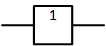
\includegraphics[scale=2.00]{img/portes_logiques/1-YES/LogicGate-YES_eur.png}

      Symbole européen
      \end{center}
    \end{minipage}
    \hfillx
    \begin{minipage}{0.50\textwidth}
      \centering
      \begin{center}

      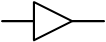
\includegraphics[scale=2.00]{img/portes_logiques/1-YES/LogicGate-YES_usa.png}

      Symbole américain
      \end{center}
    \end{minipage}

  \end{minipage}
  \hfillx
  \begin{minipage}{0.30\textwidth}
    \centering

    \begin{center}
    $ X = A $

    \medskip

    \begin{tabular}{|c"c|}
\hline
\cellcolor{black!15} \textit{A} & \cellcolor{black!15} \textit{X} \\
\thickhline
0 & \cellcolor{black!15} 0 \\ \hline
1 & \cellcolor{black!15} 1 \\ \hline
    \end{tabular}
    \end{center}

  \end{minipage}
\end{table}

Cette porte logique ne présente que peu d'intérêt.
Néanmoins, il existe des raisons techniques de s'en servir (comme réhausser un signal dans certains cas), voire, certains autres domaines indépendants de l'électronique s'appuient eux aussi sur les outils logiques et nécessitent l'équivalent d'une porte recopiant son état d'entrée.

\medskip

%\vfillFirst

\vfillLast

\subsubsection{Porte Logique NON / NOT}

Il s'agit d'une porte logique effectuant la négation de la valeur d'entrée, c'est-à-dire que l'on applique le complément à 1 sur le bit inséré en entrée.
Cette porte logique s'appelle également un \textit{inverseur} (\textit{inverter} en anglais).

\medskip

\begin{table}[!ht]
  \centering
  \begin{minipage}{0.70\textwidth}
    \centering

    Porte NON/NOT

    \medskip

    \begin{minipage}{0.50\textwidth}
      \centering
      \begin{center}
      Symbole européen (1)

      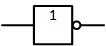
\includegraphics[scale=2.00]{img/portes_logiques/1-NOT/LogicGate-NOT_eur1.png}

      \medskip

      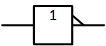
\includegraphics[scale=2.00]{img/portes_logiques/1-NOT/LogicGate-NOT_eur2.png}

      Symbole européen (2)
      \end{center}

    \end{minipage}
    \hfillx
    \begin{minipage}{0.50\textwidth}
      \centering

      \begin{center}

      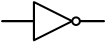
\includegraphics[scale=2.00]{img/portes_logiques/1-NOT/LogicGate-NOT_usa.png}

      Symbole américain
      \end{center}

    \end{minipage}

  \end{minipage}
  \hfillx
  \begin{minipage}{0.30\textwidth}
    \centering

    \begin{center}
    $ X = \overline{A} $

    \medskip

    \begin{tabular}{|c"c|}
\hline
\cellcolor{black!15} \textit{A} & \cellcolor{black!15} \textit{X} \\
\thickhline
0 & \cellcolor{black!15} 1 \\ \hline
1 & \cellcolor{black!15} 0 \\ \hline
    \end{tabular}
    \end{center}

  \end{minipage}
\end{table}

On notera que sur les schémas il s'agit simplement d'ajouter une bulle (ou une barre oblique sur certaines versions européennes) indiquant que l'on applique une inversion à la sortie de la porte logique.

Ainsi, la porte NON n'est qu'une porte OUI à laquelle on applique un inverseur : on effectue l'identité sur le bit de l'entrée, puis on applique le complément à 1.

Dans la représentation algébrique, on remarque qu'il s'agit d'ajouter une barre sur le bit que l'on veut inverser, tout comme dans les probabilités lorsque l'on exprime la négation d'une assertion.


%\bigskip
\clearpage

%%%%%%%%%%%%%%%%%%%%%%%%%%%%%%%%%%%%%%%%%%%%%%%%%%%%%%%%%%%%%%%%

\subsection{Portes Logiques à deux entrées}

\subsubsection{Porte Logique ET / AND}

Il s'agit d'une porte logique exigeant que les deux entrées soient simultanément activées pour que la sortie le soit.

\medskip

\begin{table}[!ht]
  \centering
  \begin{minipage}{0.70\textwidth}
    \centering

    Porte ET/AND

    \medskip

    \begin{minipage}{0.50\textwidth}
      \centering
      \begin{center}

      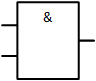
\includegraphics[scale=2.00]{img/portes_logiques/2-AND/LogicGate-AND_eur.png}

      Symbole européen
      \end{center}

    \end{minipage}
    \hfillx
    \begin{minipage}{0.50\textwidth}
      \centering

      \begin{center}

      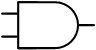
\includegraphics[scale=2.00]{img/portes_logiques/2-AND/LogicGate-AND_usa.png}

      Symbole américain
      \end{center}

    \end{minipage}

  \end{minipage}
  \hfillx
  \begin{minipage}{0.30\textwidth}
    \centering

    \begin{center}
    $ X = A \cdot B $

    \medskip

    \begin{tabular}{|c|c"c|}
\hline
\cellcolor{black!15} \textit{A} & \cellcolor{black!15} \textit{B} & \cellcolor{black!15} \textit{X} \\
\thickhline
0 & 0 & \cellcolor{black!15} 0 \\ \hline
0 & 1 & \cellcolor{black!15} 0 \\ \hline
1 & 0 & \cellcolor{black!15} 0 \\ \hline
1 & 1 & \cellcolor{black!15} 1 \\ \hline
    \end{tabular}
    \end{center}

  \end{minipage}
\end{table}

On remarquera que le symbole algébrique correspondant est un point ( $ \cdot $ ) comme pour la multiplication.
En effet, en multipliant les bits d'entrée, on obtient le bit de sortie.

\medskip

On peut interpréter cette porte de plusieurs manières.
La plus évidente consiste à indiquer que les 2 entrées doivent être actives pour que la sortie le soit également (il faut avoir 2 validations).

Une autre en logique négative serait de dire qu'il ne faut aucun désaccord pour activer la sortie.

\medskip

\vfillFirst

\vfillLast

\subsubsection{Porte Logique NON-ET / NAND}

Il s'agit d'une porte logique effectuant la négation de la porte ET, il faut donc qu'une ou moins des entrées soit activée pour que la sortie le soit.
On peut également lire cette porte comme : les deux entrées ne doivent pas être simultanément activées.

\medskip

\begin{table}[!ht]
  \centering
  \begin{minipage}{0.70\textwidth}
    \centering

    Porte NON-ET/NAND

    \medskip

    \begin{minipage}{0.50\textwidth}
      \centering
      \begin{center}
      Symbole européen (1)

      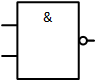
\includegraphics[scale=2.00]{img/portes_logiques/2-NAND/LogicGate-NAND_eur1.png}

      \medskip

      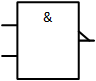
\includegraphics[scale=2.00]{img/portes_logiques/2-NAND/LogicGate-NAND_eur2.png}

      Symbole européen (2)
      \end{center}

    \end{minipage}
    \hfillx
    \begin{minipage}{0.50\textwidth}
      \centering

      \begin{center}

      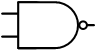
\includegraphics[scale=2.00]{img/portes_logiques/2-NAND/LogicGate-NAND_usa.png}

      Symbole américain
      \end{center}

    \end{minipage}

  \end{minipage}
  \hfillx
  \begin{minipage}{0.30\textwidth}
    \centering

    \begin{center}
    $ X = \overline{A \cdot B} $

    \medskip

    \begin{tabular}{|c|c"c|}
\hline
\cellcolor{black!15} \textit{A} & \cellcolor{black!15} \textit{B} & \cellcolor{black!15} \textit{X} \\
\thickhline
0 & 0 & \cellcolor{black!15} 1 \\ \hline
0 & 1 & \cellcolor{black!15} 1 \\ \hline
1 & 0 & \cellcolor{black!15} 1 \\ \hline
1 & 1 & \cellcolor{black!15} 0 \\ \hline
    \end{tabular}
    \end{center}

  \end{minipage}
\end{table}

Cette porte peut s'utiliser pour s'assurer que les conditions en entrées ne sont jamais vérifiées ensemble.

Au plus, une seule condition sera validée.

\medskip

On peut utiliser cette porte lorsque l'on scrute des évènements qui ne doivent surtout pas se produire simultanément.


%\medskip
\clearpage

\subsubsection{Porte Logique OU / OR}

Il s'agit d'une porte logique exigeant qu'au moins une des deux entrées soit activée pour que la sortie le soit également.

\medskip

\begin{table}[!ht]
  \centering
  \begin{minipage}{0.70\textwidth}
    \centering

    Porte OU/OR

    \medskip

    \begin{minipage}{0.50\textwidth}
      \centering
      \begin{center}

      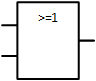
\includegraphics[scale=2.00]{img/portes_logiques/2-OR/LogicGate-OR_eur.png}

      Symbole européen
      \end{center}

    \end{minipage}
    \hfillx
    \begin{minipage}{0.50\textwidth}
      \centering

      \begin{center}

      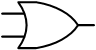
\includegraphics[scale=2.00]{img/portes_logiques/2-OR/LogicGate-OR_usa.png}

      Symbole américain
      \end{center}

    \end{minipage}

  \end{minipage}
  \hfillx
  \begin{minipage}{0.30\textwidth}
    \centering

    \begin{center}
    $ X = A + B $

    \medskip

    \begin{tabular}{|c|c"c|}
\hline
\cellcolor{black!15} \textit{A} & \cellcolor{black!15} \textit{B} & \cellcolor{black!15} \textit{X} \\
\thickhline
0 & 0 & \cellcolor{black!15} 0 \\ \hline
0 & 1 & \cellcolor{black!15} 1 \\ \hline
1 & 0 & \cellcolor{black!15} 1 \\ \hline
1 & 1 & \cellcolor{black!15} 1 \\ \hline
    \end{tabular}
    \end{center}

  \end{minipage}
\end{table}

On remarquera que le symbole algébrique correspondant est un plus ( $ + $ ) comme pour l'addition.
En effet, en additionnant les bits d'entrée, on obtient soit $ 0 $, soit une valeur supérieure à $ 0 $ qui active la sortie.
Dans la représentation européenne, on remarque également cette condition $ \geq 1 $ qui exige que la somme des entrées soit supérieure ou égale à $ 1 $.

\medskip

Cette porte peut s'utiliser dans le cas où au moins un évènement doit se produire pour activer la sortie.
Ou encore, au moins une condition doit être résolue pour activer la sortie.


\medskip

\vfillFirst

\vfillLast

\subsubsection{Porte Logique NON-OU / NOR}

Il s'agit d'une porte logique effectuant la négation de la porte OU, il faut donc qu'aucune des entrées ne soit activée pour que la sortie le soit.

\medskip

\begin{table}[!ht]
  \centering
  \begin{minipage}{0.70\textwidth}
    \centering

    Porte NON-OU/NOR

    \medskip

    \begin{minipage}{0.50\textwidth}
      \centering

      \begin{center}
      Symbole européen (1)

      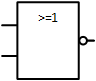
\includegraphics[scale=2.00]{img/portes_logiques/2-NOR/LogicGate-NOR_eur1.png}

      \medskip

      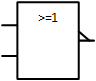
\includegraphics[scale=2.00]{img/portes_logiques/2-NOR/LogicGate-NOR_eur2.png}

      Symbole européen (2)
      \end{center}

    \end{minipage}
    \hfillx
    \begin{minipage}{0.50\textwidth}
      \centering

      \begin{center}

      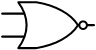
\includegraphics[scale=2.00]{img/portes_logiques/2-NOR/LogicGate-NOR_usa.png}

      Symbole américain
      \end{center}

    \end{minipage}

  \end{minipage}
  \hfillx
  \begin{minipage}{0.30\textwidth}
    \centering

    \begin{center}
    $ X = \overline{A + B} $

    \medskip

    \begin{tabular}{|c|c"c|}
\hline
\cellcolor{black!15} \textit{A} & \cellcolor{black!15} \textit{B} & \cellcolor{black!15} \textit{X} \\
\thickhline
0 & 0 & \cellcolor{black!15} 1 \\ \hline
0 & 1 & \cellcolor{black!15} 0 \\ \hline
1 & 0 & \cellcolor{black!15} 0 \\ \hline
1 & 1 & \cellcolor{black!15} 0 \\ \hline
    \end{tabular}
    \end{center}

  \end{minipage}
\end{table}

Un cas d'usage de cette porte est simplement qu'absolument aucun évènement scruté ne doit se produire pour que la sortie soit activée.

%\medskip
\clearpage

\subsubsection{Porte Logique OU Exclusif / XOR}

Il s'agit d'une porte logique exigeant qu'au plus une des deux entrées soit activée pour que la sortie le soit également.
On peut également lire cette porte comme : les deux entrées doivent être dans des états différents.

\medskip

\begin{table}[!ht]
  \centering
  \begin{minipage}{0.70\textwidth}
    \centering

    Porte OU Exclusif/XOR

    \medskip

    \begin{minipage}{0.50\textwidth}
      \centering
      \begin{center}

      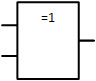
\includegraphics[scale=2.00]{img/portes_logiques/2-XOR/LogicGate-XOR_eur.png}

      Symbole européen
      \end{center}

    \end{minipage}
    \hfillx
    \begin{minipage}{0.50\textwidth}
      \centering

      \begin{center}
      Porte OU Exclusif/XOR

      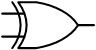
\includegraphics[scale=2.00]{img/portes_logiques/2-XOR/LogicGate-XOR_usa.png}

      Symbole américain
      \end{center}

    \end{minipage}

  \end{minipage}
  \hfillx
  \begin{minipage}{0.30\textwidth}
    \centering

    \begin{center}
    $ X = A \oplus B $

    \medskip

    \begin{tabular}{|c|c"c|}
\hline
\cellcolor{black!15} \textit{A} & \cellcolor{black!15} \textit{B} & \cellcolor{black!15} \textit{X} \\
\thickhline
0 & 0 & \cellcolor{black!15} 0 \\ \hline
0 & 1 & \cellcolor{black!15} 1 \\ \hline
1 & 0 & \cellcolor{black!15} 1 \\ \hline
1 & 1 & \cellcolor{black!15} 0 \\ \hline
    \end{tabular}
    \end{center}

  \end{minipage}
\end{table}

On remarquera que le symbole algébrique correspondant est un plus entouré ( $ \oplus $ ), car il s'agit effectivement d'une addition, mais d'une addition spéciale.
La condition exprimée est qu'une seule entrée soit active, mais ni plus ni moins.
La représentation européenne exprime effectivement cela en indiquant comme condition $ = 1 $, c'est-à-dire que la somme des entrées doit absolument être strictement égale à $ 1 $.

\medskip

Parmi les autres usages possibles, il s'agirait de vérifier exactement une seule condition pour activer la sortie.

%Ou encore, comme dans le cas du parallélisme, on peut tester si un verrou est déjà utilisé par quelqu'un.

\medskip

\vfillFirst

\vfillLast

\subsubsection{Porte Logique NON-OU Exclusif / NXOR}

La porte logique NON-OU Exclusif, aussi appelée \textit{coïncidence}, ou NXOR est la négation de la porte OU Exclusif, il faut donc qu'aucune ou les deux des entrées soient activées pour que la sortie le soit.
On peut également lire cette porte comme : les deux entrées doivent être dans le même état.
Cette porte logique s'appelle également une \textit{coïncidence}.

\medskip

\begin{table}[!ht]
  \centering
  \begin{minipage}{0.70\textwidth}
    \centering

     Porte NON-OU Exclusif/NXOR

    \medskip

    \begin{minipage}{0.50\textwidth}
      \centering
      \begin{center}
      Symbole européen (1)

      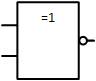
\includegraphics[scale=2.00]{img/portes_logiques/2-XNOR/LogicGate-XNOR_eur1.png}

      \medskip

      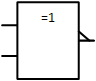
\includegraphics[scale=2.00]{img/portes_logiques/2-XNOR/LogicGate-XNOR_eur2.png}

      Symbole européen (2)
      \end{center}

    \end{minipage}
    \hfillx
    \begin{minipage}{0.50\textwidth}
      \centering

      \begin{center}

      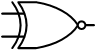
\includegraphics[scale=2.00]{img/portes_logiques/2-XNOR/LogicGate-XNOR_usa.png}

      Symbole américain
      \end{center}

    \end{minipage}

  \end{minipage}
  \hfillx
  \begin{minipage}{0.30\textwidth}
    \centering

    \begin{center}
    $ X = A \odot B = \overline{A \oplus B} $

    \medskip

    \begin{tabular}{|c|c"c|}
\hline
\cellcolor{black!15} \textit{A} & \cellcolor{black!15} \textit{B} & \cellcolor{black!15} \textit{X} \\
\thickhline
0 & 0 & \cellcolor{black!15} 1 \\ \hline
0 & 1 & \cellcolor{black!15} 0 \\ \hline
1 & 0 & \cellcolor{black!15} 0 \\ \hline
1 & 1 & \cellcolor{black!15} 1 \\ \hline
    \end{tabular}
    \end{center}

  \end{minipage}
\end{table}

On remarquera que le symbole algébrique correspondant est un point entouré ( $ \odot $ ), car il s'agit effectivement d'une multiplication, mais d'une multiplication spéciale.

%\bigskip
\clearpage

%%%%%%%%%%%%%%%%%%%%%%%%%%%%%%%%%%%%%%%%%%%%%%%%%%%%%%%%%%%%%%%%%%%%%%%%%
%%%%%%%%%%%%%%%%%%%%%%%%%%%%%%%%%%%%%%%%%%%%%%%%%%%%%%%%%%%%%%%%%%%%%%%%%
%%%%%%%%%%%%%%%%%%%%%%%%%%%%%%%%%%%%%%%%%%%%%%%%%%%%%%%%%%%%%%%%%%%%%%%%%
%%%%%%%%%%%%%%%%%%%%%%%%%%%%%%%%%%%%%%%%%%%%%%%%%%%%%%%%%%%%%%%%%%%%%%%%%

\section{Circuits Logiques \& Algèbre Booléenne}

%\bigskip
\smallskip

Les portes logiques peuvent se combiner ensemble.

Il y a néanmoins deux règles à respecter :

\begin{itemize}
\item On peut connecter à une entrée n'importe quelle autre entrée ou sortie

\item On ne peut pas connecter une sortie à une autre sortie
\end{itemize}


\begin{table}[!ht]
  \centering
  \begin{minipage}{0.45\textwidth}
    \centering

    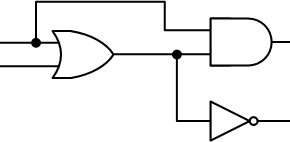
\includegraphics[width=0.45\textwidth]{img/portes_logiques/autres/connexions_autorisees_CORRECTION.png}

  \end{minipage}
  \hfillx
  \begin{minipage}{0.45\textwidth}
    \centering

     \begin{tikzpicture}
        \node[anchor=south west,inner sep=0] (image) at (0,0) {
            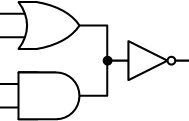
\includegraphics[width=0.40\textwidth]{img/portes_logiques/autres/connexions_interdites_CORRECTION_bis.png}
        };
        \begin{scope}[x={(image.south east)},y={(image.north west)}]
            \draw[red,line width=0.5 mm] (0, 1)--(1, 0);
            \draw[red,line width=0.5 mm] (0, 0)--(1, 1);
        \end{scope}
    \end{tikzpicture}

    %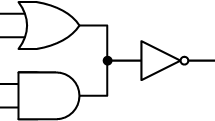
\includegraphics[width=0.40\textwidth]{img/portes_logiques/autres/connexions_interdites_CORRECTION.png}


  \end{minipage}
\end{table}

On peut simplifier les circuits logiques (en réduisant le nombre de portes logiques) grâce à l'algèbre de Boole, et, comme nous le verrons plus tard, avec les tableaux de Karnaugh.

\medskip

%%%%%%%%%%%%%%%%%%%%%%%%%%%%%%%%%%%%%%%%%%%%%%%%%%%%%%%%%%%%%%%%

\subsection{Principaux axiomes et théorèmes de l'algèbre Booléenne}

\medskip

L'algèbre Booléenne s'appuie essentiellement sur les trois opérateurs : NON, ET, OU

\begin{center}

\begin{tabular}{| c | l |}
\hline
\multirow[c]{1}{*}[0in]{Priorité} & $ A + ( B \cdot C ) = A + B \cdot C $ \\
\hline
\multirow[c]{3}{*}[0in]{NON} & $ \overline{\overline{A}} = A $     \phantom{$ \overline{\overline{\overline{A}}} $} \\
         & $ \overline{A} + A = 1 $ \\
         & $ \overline{A} \cdot A = 0 $ \\
\hline
\multirow[c]{5}{*}[0in]{ET} & $ A \cdot ( B \cdot C ) = ( A \cdot B ) \cdot C = A \cdot B \cdot C $ \\
         &  $ A \cdot B = B \cdot A $ \\
         & $ A \cdot A = A $ \\
         & $ A \cdot 1 = A $ \\
         & $ A \cdot 0 = 0 $ \\
\hline
\multirow[c]{5}{*}[0in]{OU} & $ A + ( B + C ) = ( A + B ) + C = A + B + C $ \\
         & $ A + B = B + A $ \\
         & $ A + A = A $ \\
         & $ A + 0 = A $ \\
         & $ A + 1 = 1 $ \\
\hline
\multirow[c]{8}{*}[0in]{OU EXCLUSIF} & $ A \oplus B = \overline{A} \cdot B + A \cdot \overline{B} = \overline{A} \oplus \overline{B} $   \phantom{$ \overline{\overline{A}} $} \\
         & $ \overline{A \oplus B} = A \cdot B + \overline{A} \cdot \overline{B} = \overline{A} \oplus B = A \oplus \overline{B} $ \\
         & $ A \oplus ( B \oplus C ) = ( A \oplus B ) \oplus C = A \oplus B \oplus C $ \\
         & $ A \oplus B = B \oplus A $ \\
         & $ A \oplus 0 = A $ \\
         & $ A \oplus 1 = \overline{A} $ \\
         & $ A \oplus A = 0 $ \\
         & $ A \oplus \overline{A} = 1 $ \\
\hline
\multirow[c]{2}{*}[0in]{Distributivité} & $ A \cdot ( B + C ) = A \cdot B + A \cdot C $ \\
         & $ A + B \cdot C = (A + B) \cdot (A + C) $ \\
\hline
\multirow[c]{2}{*}[0in]{Théorèmes de De Morgan} & $ \overline{A \cdot B} = \overline{A} + \overline{B} $    \phantom{$ \overline{\overline{A}} $} \\
         & $ \overline{A + B} = \overline{A} \cdot \overline{B} $ \\
\hline
\multirow[c]{2}{*}[0in]{Autres théorèmes} & Théorème 1 : $ A + A \cdot B = A $ \\
         & Théorème 2 : $ A + \overline{A} \cdot B = A + B $ \\
\hline
\end{tabular}

\smallskip

\textit{(Merci David BOUCHET pour le superbe et très complet tableau !)}

\end{center}


Il est possible de transformer un circuit de portes logiques en formule d'algèbre booléenne, et inversement, tant que les 2 règles sont respectées.

L'intérêt d'utiliser les axiomes et théorèmes est de pouvoir simplifier une formule, et donc, de produire un circuit beaucoup plus petit.


\bigskip

%%%%%%%%%%%%%%%%%%%%%%%%%%%%%%%%%%%%%%%%%%%%%%%%%%%%%%%%%%%%%%%%

\subsection{Formes canoniques}

On peut transformer une expression booléenne de plusieurs manières grâce aux formules précédentes.
Parmi ces formes, on trouve les \textit{formes canoniques}.
Les formes canoniques impliquent de détailler toutes les variables dans chaque terme de la somme ou du produit.

\smallskip

La première forme canonique est une somme de produits, tandis que la deuxième forme canonique est un produit de sommes.

\medskip

%%%%%%%%%%%%%%%%%%%%%%%%%%%%%%

%\subsubsection{Première forme canonique / Somme canonique de produits / Somme des mintermes}
\subsubsection{Mintermes / Première forme canonique / Somme canonique de produits}

% "On a trouvé une équation qui était très simple : c'était une somme de 4 produits de 3 termes chacun" -- Francis GABON

\medskip

La \textit{première forme canonique} ou \textit{somme canonique de produits} ou encore \textit{somme des mintermes} est littéralement une somme dont chaque terme est constitué de toutes les variables manipulées multipliées entre elles.
On a donc des OU dont les termes sont constitués de variables liées par des ET.

\medskip

%Un \textit{minterme} est un terme de la somme où toutes les variables sont multipliées entre elles.
Un \textit{minterme} est un produit de toutes les variables manipulées (complémentée ou non).

\medskip

Le format est du type :

$$
\sum \, X \cdot Y \cdot Z   \; \; \Rightarrow \; \;  (X \cdot Y \cdot Z) + (X \cdot \overline{Y} \cdot Z) + ...
$$

Pour obtenir une somme canonique de produits à partir d'une somme quelconque, il suffit de multiplier à chaque terme incomplet les 2 états possibles de chaque variable manquante.

\medskip

Par exemple, pour les variables A, B et C :

\smallskip

$ A \cdot B \cdot C + \overline{A} \cdot B $

\smallskip

Le terme $ \overline{A} \cdot B $ n'est pas un minterme, car il ne contient pas $ C $.

On peut obtenir la somme canonique en multipliant le dernier terme par $ ( C + \overline{C} ) $ :

\smallskip

$ A \cdot B \cdot C + \overline{A} \cdot B \bm{\cdot ( C + \overline{C} )} = A \cdot B \cdot C + \overline{A} \cdot B \bm{\cdot C} + \overline{A} \cdot B \bm{\cdot \overline{C}} $

\bigskip

Ainsi, la formule $ A \cdot B \cdot C + \overline{A} \cdot B \cdot C + \overline{A} \cdot B \cdot \overline{C} $ ne contient que des mintermes, et est la somme canonique de produits.

\smallskip

De même, si l'on avait une formule avec une quatrième variable D, il aurait fallu multiplier chaque terme de la somme où une ou des variables seraient manquantes par la ou les variables dans ses 2 états possibles.

\bigskip

On peut également retrouver une somme canonique de produits à partir d'une table de vérité (et inversement) : chaque terme de la somme correspond aux états \textit{vrais} du résultat, sachant que chaque état inversé d'une variable correspond à un $ 0 $.

\begin{center}
$ X = A \cdot B \cdot C + \overline{A} \cdot B \cdot C + \overline{A} \cdot B \cdot \overline{C} $

\smallskip

$ A \cdot B \cdot C  \; \; \Rightarrow \; \;  A = 1 \; , \; B = 1 \; , \; C = 1 $

$ \overline{A} \cdot B \cdot C  \; \; \Rightarrow \; \;  \overline{A} = 0 \; , \; B = 1 \; , \; C = 1 $

$ \overline{A} \cdot B \cdot \overline{C}  \; \; \Rightarrow \; \;  \overline{A} = 0 \; , \; B = 1 \; , \; \overline{C} = 0 $

\medskip

\begin{tabular}{| c | c | c || c | l }
\cline{0-3}
\cellcolor{black!15} \textbf{A} & \cellcolor{black!15} \textbf{B} & \cellcolor{black!15} \textbf{C}  &  \cellcolor{black!15} \textbf{X}  & \\
\cline{0-3}
0 & 0 & 0  &  \cellcolor{black!15} 0  & \\ \cline{0-3}
0 & 0 & 1  &  \cellcolor{black!15} 0  & \\ \cline{0-3}
0 & 1 & 0  &  \cellcolor{black!15} 1  & $ \leftarrow \overline{A} \cdot B \cdot \overline{C} $ \\ \cline{0-3}
0 & 1 & 1  &  \cellcolor{black!15} 1  & $ \leftarrow \overline{A} \cdot B \cdot C $ \\ \cline{0-3}
1 & 0 & 0  &  \cellcolor{black!15} 0  & \\ \cline{0-3}
1 & 0 & 1  &  \cellcolor{black!15} 0  & \\ \cline{0-3}
1 & 1 & 0  &  \cellcolor{black!15} 0  & \\ \cline{0-3}
1 & 1 & 1  &  \cellcolor{black!15} 1  & $ \leftarrow  A \cdot B \cdot C $ \\ \cline{0-3}
\end{tabular}
\end{center}

\medskip

%%%%%%%%%%%%%%%%%%%%%%%%%%%%%%

%\subsubsection{Deuxième forme canonique / Produit canonique de sommes / Produit des maxtermes}
\subsubsection{Maxtermes / Seconde forme canonique / Produit canonique de sommes}

\medskip

La \textit{seconde forme canonique} ou \textit{produit canonique de sommes} ou encore \textit{produit des maxtermes} est littéralement un produit dont chaque terme est constitué de toutes les variables manipulées additionnées entre elles.
On a donc des ET dont les termes sont constitués de variables liées par des OU.

\medskip

%Un \textit{maxterme} est un terme du produit où toutes les variables sont additionnes entre elles.
Un \textit{maxterme} est une somme de toutes les variables manipulées (complémentée ou non).

\medskip

Le format est du type :

$$
\prod \, X + Y + Z   \; \; \Rightarrow \; \;  (X + Y + Z) \cdot (X + \overline{Y} + Z) \cdot 	...
$$

Pour obtenir un produit canonique de sommes à partir d'un produit quelconque, il suffit d'additioner à chaque terme incomplet les 2 états possibles de chaque variable manquante.

\medskip

Par exemple, pour les variables A, B et C :

\smallskip

$ ( A + B + C ) \cdot ( \overline{A} + B ) $

\smallskip

Le terme $ \overline{A} + B $ n'est pas un maxterme, car il ne contient pas $ C $.

On peut obtenir le produit canonique en ajoutant au dernier terme $ ( C \cdot \overline{C} ) $ :

\smallskip

$ ( A + B + C ) \cdot ( \overline{A} + B \bm{+ ( C + \overline{C} )} ) = ( A + B + C ) \cdot ( \overline{A} + B \bm{+ C} ) \cdot ( \overline{A} + B \bm{+ \overline{C}} ) $

\bigskip

Ainsi, la formule $ ( A + B + C ) \cdot ( \overline{A} + B + C ) \cdot ( \overline{A} + B + \overline{C} ) $ ne contient que des maxtermes, et est le produit canonique de sommes.

\smallskip

De même, si l'on avait une formule avec une quatrième variable D, il aurait fallu ajouter, à chaque terme de la somme où une ou des variables seraient manquantes, la ou les variables dans ses 2 états possibles.

\bigskip

On peut également retrouver un produit canonique de sommes à partir d'une table de vérité (et inversement) : chaque terme du produit correspond aux états \textit{faux} du résultat, sachant que chaque état inversé d'une variable correspond à un $ 1 $.

\begin{center}
$ X = (A + B + C) \cdot (\overline{A} + B + C) \cdot (\overline{A} + B + \overline{C}) $

\smallskip

$ A + B + C  \; \; \Rightarrow \; \;  A = 0 \; , \; B = 0 \; , \; C = 0 $

$ \overline{A} + B + C  \; \; \Rightarrow \; \;  \overline{A} = 1 \; , \; B = 0 \; , \; C = 0 $

$ \overline{A} + B + \overline{C}  \; \; \Rightarrow \; \;  \overline{A} = 1 \; , \; B = 0 \; , \; \overline{C} = 1 $

\medskip

\begin{tabular}{| c | c | c || c | l }
\cline{0-3}
\cellcolor{black!15} \textbf{A} & \cellcolor{black!15} \textbf{B} & \cellcolor{black!15} \textbf{C}  &  \cellcolor{black!15} \textbf{X}  & \\
\cline{0-3}
0 & 0 & 0  &  \cellcolor{black!15} 0  & $ \leftarrow  A + B + C $ \\ \cline{0-3}
0 & 0 & 1  &  \cellcolor{black!15} 1  & \\ \cline{0-3}
0 & 1 & 0  &  \cellcolor{black!15} 1  & \\ \cline{0-3}
0 & 1 & 1  &  \cellcolor{black!15} 1  & \\ \cline{0-3}
1 & 0 & 0  &  \cellcolor{black!15} 0  & $ \leftarrow \overline{A} + B + C $ \\ \cline{0-3}
1 & 0 & 1  &  \cellcolor{black!15} 0  & $ \leftarrow \overline{A} + B + \overline{C} $ \\ \cline{0-3}
1 & 1 & 0  &  \cellcolor{black!15} 1  & \\ \cline{0-3}
1 & 1 & 1  &  \cellcolor{black!15} 1  & \\ \cline{0-3}
\end{tabular}
\end{center}

\bigskip

Pour construire les maxtermes, il s'agit de suivre la logique inverse des mintermes.

\medskip

On peut également le voir comme la recherche de l'état absorbant pour l'opération principale :

\begin{itemize}
\item dans les \textit{mintermes}, c'est un OU/l'addition qui est l'opération principale, donc un état \linebreak \textit{vrai}/1 est absorbant : on va chercher tous les états absorbants pouvant renvoyer 1
\item dans les \textit{maxtermes}, c'est un ET/la multiplication qui est l'opération principale, donc un état \textit{faux}/0 est absorbant : on va chercher tous les états absorbants pouvant renvoyer 0
\end{itemize}

De fait, passer d'une forme canonique à l'autre revient à sélectionner les résultats inverses, en appliquant également l'inverse sur l'état des variables.


\medskip

%%%%%%%%%%%%%%%%%%%%%%%%%%%%%%%%%%%%%%%%%%%%%%%%%%%%%%%%%%%%%%%%

\subsection{Tableaux de Karnaugh}

\medskip

Pour simplifier les expressions booléennes, on doit s'appuyer sur les formules présentées plus tôt.
Néanmoins, il existe une méthode graphique permettant de résoudre cela : les \textit{tableaux de Karnaugh} ou \textit{diagrammes de Karnaugh}.

\medskip

\`A partir d'une table de vérité, on va construire un tableau de Karnaugh et y dessiner les plus grands groupes de 1 alignés sous forme de rectangles ou carrés.
Ces regroupements permettent de déterminer quelles variables ou états sont constamment vérifiés et ne nécessitent donc pas d'être écrits dans la formule finale.
La formule finale n'est donc quasiment jamais une forme canonique.

\medskip

%%%%%%%%%%%%%%%%%%%%%%%%%%%%%%

\subsubsection{Construction d'une table de vérité}

\medskip

Pour construire un tableau de Karnaugh, on doit d'abord construire la table de vérité.
Cette table s'obtient simplement en testant l'ensemble des combinaisons possibles des variables composant une formule.

\medskip

$$
X = A \cdot B + \overline{B} \cdot \overline{C} + A \cdot \overline{B} \cdot \overline{C} + \overline{A} \cdot C
$$

\begin{center}
\begin{tabular}{| c | c | c || c | m{0.5cm} l }
\cline{0-3}
\cellcolor{black!15} \textbf{A} & \cellcolor{black!15} \textbf{B} & \cellcolor{black!15} \textbf{C}  &  \cellcolor{black!15} \textbf{X}  & & \\
\cline{0-3}
0 & 0 & 0  &  \cellcolor{black!15} 1  & & $ X = \textcolor{gray}{A \cdot B + \textcolor{black}{\overline{B} \cdot \overline{C}} + A \cdot \overline{B} \cdot \overline{C} + \overline{A} \cdot C} $ \\ \cline{0-3}
0 & 0 & 1  &  \cellcolor{black!15} 1  & & $ X = \textcolor{gray}{A \cdot B + \overline{B} \cdot \overline{C} + A \cdot \overline{B} \cdot \overline{C} + \textcolor{black}{\overline{A} \cdot C}} $ \\ \cline{0-3}
0 & 1 & 0  &  \cellcolor{black!15} 0  & & \\ \cline{0-3}
0 & 1 & 1  &  \cellcolor{black!15} 1  & & $ X = \textcolor{gray}{A \cdot B + \overline{B} \cdot \overline{C} + A \cdot \overline{B} \cdot \overline{C} + \textcolor{black}{\overline{A} \cdot C}} $ \\ \cline{0-3}
1 & 0 & 0  &  \cellcolor{black!15} 1  & & $ X = \textcolor{gray}{A \cdot B + \textcolor{black}{\overline{B} \cdot \overline{C}} + \textcolor{black}{A \cdot \overline{B} \cdot \overline{C}} + \overline{A} \cdot C} $ \\ \cline{0-3}
1 & 0 & 1  &  \cellcolor{black!15} 0  & & \\ \cline{0-3}
1 & 1 & 0  &  \cellcolor{black!15} 1  & & $ X = \textcolor{gray}{\textcolor{black}{A \cdot B} + \overline{B} \cdot \overline{C} + A \cdot \overline{B} \cdot \overline{C} + \overline{A} \cdot C} $ \\ \cline{0-3}
1 & 1 & 1  &  \cellcolor{black!15} 1  & & $ X = \textcolor{gray}{\textcolor{black}{A \cdot B} + \overline{B} \cdot \overline{C} + A \cdot \overline{B} \cdot \overline{C} + \overline{A} \cdot C} $ \\ \cline{0-3}
\end{tabular}
\end{center}


\medskip

%%%%%%%%%%%%%%%%%%%%%%%%%%%%%%

\subsubsection{Transformation d'une table de vérité en tableau de Karnaugh}

\medskip

Une fois la table de vérité trouvée, il faut la transformer en tableau de Karnaugh en respectant le format des états des variables.

\smallskip

Chaque côté du tableau représente $ \frac{N}{2} $ variables, et éventuellement $ \frac{N}{2} - 1 $ variables si leur nombre est impair.
Par exemple, lorsque la formule concerne 4 variables, on va construire un tableau \og carré \fg{} de 2 variables sur 2, tandis que si la formule concerne 3 variables, on va construire un tableau \og rectangulaire \fg{} de 1 variable sur 2.

\smallskip

Les variables observées doivent être triées dans des états respectant strictement le code Gray : $ 00 $, $ 01 $, $ 11 $, $ 10 $, ...

\medskip

\begin{table}[!ht]
  \centering
  \begin{minipage}{0.30\textwidth}
    \centering

\begin{tabular}{| c | c | c || c |}
\hline
\cellcolor{black!15} \textbf{A} & \cellcolor{black!15} \textbf{B} & \cellcolor{black!15} \textbf{C}  &  \cellcolor{black!15} \textbf{X} \\
\hline
0 & 0 & 0  &  \cellcolor{black!15} 1 \\ \hline
0 & 0 & 1  &  \cellcolor{black!15} 1 \\ \hline
0 & 1 & 0  &  \cellcolor{black!15} 0 \\ \hline
0 & 1 & 1  &  \cellcolor{black!15} 1 \\ \hline
1 & 0 & 0  &  \cellcolor{black!15} 1 \\ \hline
1 & 0 & 1  &  \cellcolor{black!15} 0 \\ \hline
1 & 1 & 0  &  \cellcolor{black!15} 1 \\ \hline
1 & 1 & 1  &  \cellcolor{black!15} 1 \\ \hline
\end{tabular}

  \end{minipage}
  \hfillx
  \begin{minipage}{0.65\textwidth}
    \centering

$ X = A \cdot B + \overline{B} \cdot \overline{C} + A \cdot \overline{B} \cdot \overline{C} + \overline{A} \cdot C $

\medskip

La formule contenant 3 variables A, B et C donnera :

\bigskip

\begin{tabular}{R{0.5cm}  | c | c | c | c | c |  L{3cm} }
\multicolumn{2}{c}{ } & \multicolumn{4}{c}{\textbf{BC}} \\
\cline{2-6}
 & \cellcolor{black!65} \textbf{X} & \cellcolor{black!15} \textbf{00} & \cellcolor{black!15} \textbf{01} & \cellcolor{black!15} \textbf{11} & \cellcolor{black!15} \textbf{10}  & $ \leftarrow $ Code Gray \\
\cline{2-6}
\multirow{2}{*}{\textbf{A}} & \cellcolor{black!15} \textbf{0} & 1 & 1 & 1 & 0  & \\
\cline{2-6}
 & \cellcolor{black!15} \textbf{1} & 1 & 0 & 1 & 1  & \\
\cline{2-6}
\multicolumn{1}{c}{ } & \multicolumn{1}{c}{$ \uparrow $} & \multicolumn{4}{c}{ } \\
\multicolumn{3}{c}{Code Gray} & \multicolumn{3}{c}{ } \\
\end{tabular}

  \end{minipage}
\end{table}

\medskip

%%%%%%%%%%%%%%%%%%%%%%%%%%%%%%

\subsubsection{Recherche de groupes dans le tableau de Karnaugh}

\medskip

Une fois le tableau construit, on peut rechercher les groupes de $ 1 $ et les encercler en respectant certaines règles :

\begin{itemize}
\item ensemble des $ 1 $ doivent être dans un ou plusieurs groupes
\item Le nombre de cases dans un même groupe doit être une puissance de 2
\item Les cercles doivent être de taille maximale
\item Le nombre de cercles doit être minimum
\end{itemize}

Les groupes peuvent partager quelques éléments, mais ils doivent rester de taille maximum sans englober intégralement un autre groupe.
On peut disposer de groupes ne contenant qu'un seul élément.

\medskip

\begin{table}[!ht]
  \centering
  \begin{minipage}{0.33\textwidth}
    \centering

%\begin{tabular}{R{0.5cm}  | c | c | c | c | c |}
%\multicolumn{1}{c}{ } & \multicolumn{4}{c}{\textbf{BC}} \\
%\cline{2-6}
% & \textbf{X} & \textbf{00} & \textbf{01} & \textbf{11} & \textbf{10}\\
%\cline{2-6}
%\multirow{2}{*}{\textbf{A}} & \textbf{0} & 1 & 1 & 1 & 0 \\
%\cline{2-6}
% & \textbf{1} & 1 & 0 & 1 & 1 \\
%\cline{2-6}
%\end{tabular}

\begin{tabular}{R{0.5cm}  | c | c | c | c | c |}
\multicolumn{2}{c}{ } & \multicolumn{4}{c}{\textbf{BC}} \\
\cline{2-6}
 & \cellcolor{black!45} \textbf{X} & \cellcolor{black!15} \textbf{00} & \cellcolor{black!15} \textbf{01} & \cellcolor{black!15} \textbf{11} & \cellcolor{black!15} \textbf{10} \\
\cline{2-6}
\multirow{2}{*}{\textbf{A}} & \cellcolor{black!15} \textbf{0} & \tikzmarknode{g1A}{1} & \tikzmarknode{g2A}{1} & \tikzmarknode{g2B}{1} & 0 \\
\cline{2-6}
 & \cellcolor{black!15} \textbf{1} & \tikzmarknode{g1B}{1} & 0 & \tikzmarknode{g3A}{1} & \tikzmarknode{g3B}{1} \\
\cline{2-6}
\end{tabular}

\tikz[remember picture, overlay]{
%%  \node[draw, rounded rectangle, fit=(g1A.center) (g1B.center)] {};
%%  \node[draw, rounded rectangle, fit=(g2A.center) (g2B.center)] {};
%%  \node[draw, rounded rectangle, fit=(g3A.center) (g3B.center)] {};
%  \node[draw, rounded rectangle, inner sep=3pt, minimum size=3mm, fit=(g1A.north) (g1B.south)] {};
%  \node[draw, rounded rectangle, inner sep=3pt, minimum size=3mm, fit=(g2A.west) (g2B.east)] {};
%  \node[draw, rounded rectangle, inner sep=3pt, minimum size=3mm, fit=(g3A.west) (g3B.east)] {};

\tikzstyle{surround} = [thick, draw=middarkgreen, rounded corners=1mm]
            \begin{pgfonlayer}{background}
                %This is working well with: scale = 1 / 0.4 = 2.5
                \node[surround, scale=1] (background) [fit = (g1A.north west) (g1B.south east) (g1A.north east) ] {};
%                \node[surround, scale=1] (background) [fit = (g2A.north west) (g2B.south east) (g2A.north east) ] {};
%                \node[surround, scale=1] (background) [fit = (g3A.north west) (g3B.south east) (g3A.north east) ] {};
            \end{pgfonlayer}

\tikzstyle{surround} = [thick, draw=red, rounded corners=1mm]
            \begin{pgfonlayer}{background}
                %This is working well with: scale = 1 / 0.4 = 2.5
%                \node[surround, scale=1] (background) [fit = (g1A.north west) (g1B.south east) (g1A.north east) ] {};
                \node[surround, scale=1] (background) [fit = (g2A.north west) (g2B.south east) (g2A.north east) ] {};
%                \node[surround, scale=1] (background) [fit = (g3A.north west) (g3B.south east) (g3A.north east) ] {};
            \end{pgfonlayer}

\tikzstyle{surround} = [thick, draw=blue, rounded corners=1mm]
            \begin{pgfonlayer}{background}
                %This is working well with: scale = 1 / 0.4 = 2.5
%                \node[surround, scale=1] (background) [fit = (g1A.north west) (g1B.south east) (g1A.north east) ] {};
%                \node[surround, scale=1] (background) [fit = (g2A.north west) (g2B.south east) (g2A.north east) ] {};
                \node[surround, scale=1] (background) [fit = (g3A.north west) (g3B.south east) (g3A.north east) ] {};
            \end{pgfonlayer}

}


  \end{minipage}
  \hfillx
  \begin{minipage}{0.22\textwidth}
    \centering

\begin{center}
Groupe 1 (vert) :

\medskip

\begin{tabular}{R{0.5cm}  | c | c |  L{0.5cm}}
\multicolumn{2}{c}{ } & \multicolumn{1}{c}{\textbf{BC}} & \\
\cline{2-3}
 & \cellcolor{black!45} \textbf{ } & \cellcolor{black!15} \textbf{00} & \\
\cline{2-3}
\multirow{2}{*}{\textbf{A}} & \cellcolor{black!15} \textbf{0} & 1 & \\
\cline{2-3}
 & \cellcolor{black!15} \textbf{1} & 1 & \\
\cline{2-3}
\end{tabular}
\end{center}

  \end{minipage}
  \hfillx
  \begin{minipage}{0.22\textwidth}
    \centering

\begin{center}
Groupe 2 (rouge) :

\medskip

\begin{tabular}{R{0.5cm}  | c | c | c |}
\multicolumn{2}{c}{ } & \multicolumn{2}{c}{\textbf{BC}} \\
\cline{2-4}
 & \cellcolor{black!45} \textbf{ } & \cellcolor{black!15} \textbf{01} & \cellcolor{black!15} \textbf{11} \\
\cline{2-4}
\textbf{A} & \cellcolor{black!15} \textbf{0} & 1 & 1 \\
\cline{2-4}
\end{tabular}
\end{center}

  \end{minipage}
  \hfillx
  \begin{minipage}{0.22\textwidth}
    \centering

\begin{center}
Groupe 3 (bleu) :

\medskip

\begin{tabular}{R{0.5cm}  | c | c | c |}
\multicolumn{2}{c}{ } & \multicolumn{2}{c}{\textbf{BC}} \\
\cline{2-4}
 & \cellcolor{black!45} \textbf{ } & \cellcolor{black!15} \textbf{11} & \cellcolor{black!15} \textbf{10} \\
\cline{2-4}
\textbf{A} & \cellcolor{black!15} \textbf{1} & 1 & 1 \\
\cline{2-4}
\end{tabular}
\end{center}

  \end{minipage}
\end{table}


\medskip

Chaque groupe correspond à un terme de la formule optimisée.
Chaque terme est un produit (un ET) de variables, et les termes sont sommés ensemble.

Une fois les groupes établis, il faut donc prendre chacun des groupes et le transformer en un terme en respectant ces règles :

\begin{itemize}
\item Une variable qui change d'état est ignorée/n'apparait pas dans le terme
\item Une variable qui reste à 0 doit être retranscrite comme complémentée (avec une barre)
\item Une variable qui reste à 1 doit être retranscrite normalement (sans barre)
\end{itemize}

\medskip


\begin{table}[!ht]
  \centering
  \begin{minipage}{0.30\textwidth}
    \centering

\begin{center}
Groupe 1 (vert) :

\medskip

\begin{tabular}{R{0.5cm}  | c | c |  L{0.5cm}}
\multicolumn{2}{c}{ } & \multicolumn{1}{c}{\textbf{BC}} & \\
\cline{2-3}
 & \cellcolor{black!45} \textbf{ } & \cellcolor{black!15} \textbf{00} & \\
\cline{2-3}
\multirow{2}{*}{\textbf{A}} & \cellcolor{black!15} \textbf{0} & 1 & \\
\cline{2-3}
 & \cellcolor{black!15} \textbf{1} & 1 & \\
\cline{2-3}
\end{tabular}
\end{center}


\begin{itemize}
\item A varie entre 0 et 1
\item B reste à 0
\item C reste à 0
\end{itemize}

\smallskip

$ \Rightarrow \overline{B} \cdot \overline{C} $

  \end{minipage}
  \hfillx
  \begin{minipage}{0.30\textwidth}
    \centering

\begin{center}
Groupe 2 (rouge) :

\medskip

\begin{tabular}{R{0.5cm}  | c | c | c |  L{0.5cm}}
\multicolumn{2}{c}{ } & \multicolumn{2}{c}{\textbf{BC}} & \\
\cline{2-4}
 & \cellcolor{black!45} \textbf{ } & \cellcolor{black!15} \textbf{01} & \cellcolor{black!15} \textbf{11} & \\
\cline{2-4}
\textbf{A} & \cellcolor{black!15} \textbf{0} & 1 & 1 & \\
\cline{2-4}
\end{tabular}
\end{center}

\medskip

\begin{itemize}
\item A reste à 0
\item B varie entre 0 et 1
\item C reste à 1
\end{itemize}

\smallskip

$ \Rightarrow \overline{A} \cdot C $

  \end{minipage}
  \hfillx
  \begin{minipage}{0.30\textwidth}
    \centering

\begin{center}
Groupe 3 (bleu) :

\medskip

\begin{tabular}{R{0.5cm}  | c | c | c |  L{0.5cm}}
\multicolumn{2}{c}{ } & \multicolumn{2}{c}{\textbf{BC}} & \\
\cline{2-4}
 & \cellcolor{black!45} \textbf{ } & \cellcolor{black!15} \textbf{11} & \cellcolor{black!15} \textbf{10} & \\
\cline{2-4}
\textbf{A} & \cellcolor{black!15} \textbf{1} & 1 & 1 & \\
\cline{2-4}
\end{tabular}
\end{center}

\medskip

\begin{itemize}
\item A reste à 1
\item B reste à 1
\item C varie entre 0 et 1
\end{itemize}

\smallskip

$ \Rightarrow A \cdot B $

  \end{minipage}
\end{table}


\medskip


On reconstruit donc la somme de produits suivante :

\begin{center}
%$ \overline{B} \cdot \overline{C} \; \; + \; \; \overline{A} \cdot C \; \; + \; \; A \cdot B $
%
%\smallskip
%
%$ = A \cdot B \; \; + \; \; \overline{B} \cdot \overline{C} \; \; + \; \; \overline{A} \cdot C $
$ A \cdot B \; \; + \; \; \overline{B} \cdot \overline{C} \; \; + \; \; \overline{A} \cdot C $
\end{center}


Ce qui correspond à une versions simplifiée de la formule initiale :

\begin{center}
$ X \; \; = \; \; A \cdot B + \overline{B} \cdot \overline{C} + A \cdot \overline{B} \cdot \overline{C} + \overline{A} \cdot C \; \; = \; \; A \cdot B + \overline{B} \cdot \overline{C} + \overline{A} \cdot C $
\end{center}

\medskip

On peut donc en déduire un circuit logique simplifié en quantité de portes logiques (et donc une réduction de la quantité de composants requis et d'énergie pour les alimenter et les faire changer d'état).


\bigskip


Attention, le tableau de Karnaugh peut être construit dans n'importe quel ordre : $ A \times BC = AB \times C = AC \times B $.
Ceci implique que les \og bords \fg{} du tableau se recoupent : on peut construire un carré à partir des valeurs dans les coins.




%%%%%%%%%%%%%%%%%%%%%%%%%%%%%%%%%%%%%%%%%%%%%%%%%%%%%%%%%%%%%%%%%%%%%%%%%
%%%%%%%%%%%%%%%%%%%%%%%%%%%%%%%%%%%%%%%%%%%%%%%%%%%%%%%%%%%%%%%%%%%%%%%%%
%%%%%%%%%%%%%%%%%%%%%%%%%%%%%%%%%%%%%%%%%%%%%%%%%%%%%%%%%%%%%%%%%%%%%%%%%
%%%%%%%%%%%%%%%%%%%%%%%%%%%%%%%%%%%%%%%%%%%%%%%%%%%%%%%%%%%%%%%%%%%%%%%%%

\bigskip

\vfillFirst

\vfillLast


\begin{center}
\textit{Ce document et ses illustrations ont été réalisés par Fabrice BOISSIER en novembre 2023. \newline
Le contenu est très inspiré des supports de cours d'Anne-Sophie DUJARDIN et David BOUCHET.}

%\textit{(dernière mise à jour septembre 2023)}
\end{center}

\end{document}
